\documentclass{beamer}
\usepackage[utf8]{inputenc}
\usepackage{graphicx, epsfig}
\usepackage{amsmath,mathrsfs,amsfonts,amssymb}
\usepackage{floatflt}
\usepackage{epic,ecltree}
\usepackage{mathtext}
\usepackage{fancybox}
\usepackage{fancyhdr}
\usepackage{multirow}
\usepackage{enumerate}
\usepackage{epstopdf}
\usepackage{multicol}
\usepackage{algorithm}
\usepackage[noend]{algorithmic}
\usepackage{tikz}
\usepackage{blindtext}
\usetheme{default}%{Singapore}%{Warsaw}%{Warsaw}%{Darmstadt}
\usecolortheme{default}

\setbeamerfont{title}{size=\Huge}
\setbeamertemplate{footline}[page number]{}

\setbeamertemplate{section in toc}[sections numbered]


\makeatletter
\newcommand\HUGE{\@setfontsize\Huge{35}{40}}
\makeatother    

\setbeamerfont{title}{size=\HUGE}
\beamertemplatenavigationsymbolsempty

% latin bold lower
\newcommand{\ba}{\mathbf{a}} 
\newcommand{\bc}{\mathbf{c}} 
\newcommand{\be}{\mathbf{e}} 
\newcommand{\bff}{\mathbf{f}} % \bf - for bold type
\newcommand{\bg}{\mathbf{g}} 
\newcommand{\bh}{\mathbf{h}} 
\newcommand{\bp}{\mathbf{p}} 
\newcommand{\bq}{\mathbf{q}} 
\newcommand{\bt}{\mathbf{t}} 
\newcommand{\bs}{\mathbf{s}} 
\newcommand{\bu}{\mathbf{u}} 
\newcommand{\bv}{\mathbf{v}} 
\newcommand{\bw}{\mathbf{w}} 
\newcommand{\bx}{\mathbf{x}} 
\newcommand{\by}{\mathbf{y}} 
\newcommand{\bz}{\mathbf{z}} 

% latin bold upper
\newcommand{\bA}{\mathbf{A}} 
\newcommand{\bB}{\mathbf{B}} 
\newcommand{\bC}{\mathbf{C}} 
\newcommand{\bG}{\mathbf{G}} 
\newcommand{\bI}{\mathbf{I}} 
\newcommand{\bJ}{\mathbf{J}} 
\newcommand{\bL}{\mathbf{L}} 
\newcommand{\bM}{\mathbf{M}} 
\newcommand{\bP}{\mathbf{P}}
\newcommand{\bQ}{\mathbf{Q}} 
\newcommand{\bR}{\mathbf{R}} 
\newcommand{\bT}{\mathbf{T}} 
\newcommand{\bU}{\mathbf{U}} 
\newcommand{\bV}{\mathbf{V}} 
\newcommand{\bW}{\mathbf{W}} 
\newcommand{\bX}{\mathbf{X}} 
\newcommand{\bY}{\mathbf{Y}} 
\newcommand{\bZ}{\mathbf{Z}} 

% latin cal upper
\newcommand{\cF}{\mathcal{F}} 
\newcommand{\cG}{\mathcal{G}} 
\newcommand{\cI}{\mathcal{I}} 
\newcommand{\cL}{\mathcal{L}} 
\newcommand{\cM}{\mathcal{M}} 
\newcommand{\cN}{\mathcal{N}} 
\newcommand{\cP}{\mathcal{P}} 
\newcommand{\cS}{\mathcal{S}} 
\newcommand{\cT}{\mathcal{T}} 
\newcommand{\cW}{\mathcal{W}} 
\newcommand{\cX}{\mathcal{X}} 
\newcommand{\cZ}{\mathcal{Z}} 

% latin bb upper
\newcommand{\bbE}{\mathbb{E}} 
\newcommand{\bbI}{\mathbb{I}} 
\newcommand{\bbP}{\mathbb{P}} 
\newcommand{\bbR}{\mathbb{R}} 

% greek bold lower
\newcommand{\bepsilon}{\boldsymbol{\epsilon}} 
\newcommand{\btheta}{\boldsymbol{\theta}} 
\newcommand{\blambda}{\boldsymbol{\lambda}} 
\newcommand{\bpi}{\boldsymbol{\pi}} 
\newcommand{\bmu}{\boldsymbol{\mu}} 
\newcommand{\bsigma}{\boldsymbol{\sigma}} 
\newcommand{\bphi}{\boldsymbol{\phi}} 

% greek bold upper
\newcommand{\bSigma}{\boldsymbol{\Sigma}} 

\DeclareMathOperator*{\argmin}{arg\,min}
\DeclareMathOperator*{\argmax}{arg\,max}
\newcommand{\createdgmtitle}[1]{\title[\hbox to 56mm{Deep Generative Models  \hfill\insertframenumber\,/\,\inserttotalframenumber}]
	{\vspace{1cm} \\ \textbf{Deep Generative Models} \\ {\Huge Lecture #1}}
	\author{Roman Isachenko}
		\institute{
\includegraphics[width=0.7cm]{../utils/aimasterslogo} \LARGE{AI Masters}}
	\date{2025, Spring}
}

\usepackage{tikz}
\usetikzlibrary{arrows,shapes,positioning,shadows,trees}

\newcommand\myfootnote[1]{%
  \tikz[remember picture,overlay]
  \draw (current page.south west) +(1in + \oddsidemargin,0.5em)
  node[anchor=south west,inner sep=0pt]{\parbox{\textwidth}{%
      \rlap{\rule{10em}{0.4pt}}\raggedright\scriptsize \textit{#1}}};}

\newcommand\myfootnotewithlink[2]{%
  \tikz[remember picture,overlay]
  \draw (current page.south west) +(1in + \oddsidemargin,0.5em)
  node[anchor=south west,inner sep=0pt]{\parbox{\textwidth}{%
      \rlap{\rule{10em}{0.4pt}}\raggedright\scriptsize\href{#1}{\textit{#2}}}};}
      
\AtBeginSection[]
      {
      	\begin{frame}{Outline}
      		\tableofcontents[currentsection]
      	\end{frame}
      }
      \AtBeginSubsection[]{
      	\begin{frame}{Outline}
      		\tableofcontents[currentsection,currentsubsection]
      	\end{frame}
}
\createdgmtitle{4}
%--------------------------------------------------------------------------------
\begin{document}
%--------------------------------------------------------------------------------
\begin{frame}[noframenumbering,plain]
	%\thispagestyle{empty}
	\titlepage
\end{frame}
%=======
\begin{frame}{Recap of previous lecture}
	\begin{block}{Forward KL for flow model}
	  	\vspace{-0.1cm}
		\[
			\log p(\bx|\btheta) = \log p(\bff_{\btheta}(\bx)) + \log  |\det (\bJ_\bff)|
		\]
		\vspace{-0.3cm}
	\end{block}
	\begin{block}{Reverse KL for flow model}
  		\vspace{-0.1cm}
		\[
			KL(p || \pi)  = \bbE_{p(\bz)} \left[  \log p(\bz) -  \log |\det (\bJ_\bg)| - \log \pi(\bg_{\btheta}(\bz)) \right]
		\]
		\vspace{-0.5cm}
	\end{block}
	\begin{block}{Flow KL duality}
	  	\vspace{-0.3cm}
		\[
			\argmin_{\btheta} KL(\pi(\bx) || p(\bx | \btheta)) = \argmin_{\btheta} KL(p(\bz | \btheta) || p(\bz))
		\]
		\vspace{-0.3cm}
		\begin{itemize}
			\item $p(\bz)$ is a base distribution; $\pi(\bx)$ is a data distribution;
			\item $\bz \sim p(\bz)$, $\bx = \bg_{\btheta}(\bz)$, $\bx \sim p(\bx| \btheta)$;
			\item $\bx \sim \pi(\bx)$, $\bz = \bff_{\btheta}(\bx)$, $\bz \sim p(\bz | \btheta)$.
		\end{itemize}
	\end{block}
	\myfootnotewithlink{https://arxiv.org/abs/1912.02762}{Papamakarios G. et al. Normalizing flows for probabilistic modeling and inference, 2019} 
\end{frame}
%=======
\begin{frame}{Recap of previous lecture}
	\begin{block}{Posterior distribuiton (Bayes theorem)}
		\[
			p(\btheta | \bx) = \frac{p(\bx | \btheta) p(\btheta)}{p(\bx)} = \frac{p(\bx | \btheta) p(\btheta)}{\int p(\bx | \btheta) p(\btheta) d \btheta} 
		\]
		\begin{itemize}
			\item $\bx$ -- observed variables;
			\item $\btheta$ -- unobserved variables (latent variables/parameters);
			\item $p(\bx | \btheta)$ -- likelihood;
			\item $p(\bx) = \int p(\bx | \btheta) p(\btheta) d \btheta$ -- evidence;
			\item $p(\btheta)$ -- prior distribution;
			\item $p(\btheta | \bx)$ -- posterior distribution.
		\end{itemize}
	\end{block}
\end{frame}
%=======
\begin{frame}{Recap of previous lecture}
	\begin{block}{Latent variable models (LVM)}
		\vspace{-0.3cm}
		\[
		p(\bx | \btheta) = \int p(\bx, \bz | \btheta) d\bz = \int p(\bx | \bz, \btheta) p(\bz) d\bz.
		\]
	\end{block}
	\begin{block}{MLE problem for LVM}
		\vspace{-0.7cm}
		\begin{multline*}
			\btheta^* = \argmax_{\btheta} \log p(\bX| \btheta) = \argmax_{\btheta} \sum_{i=1}^n \log p(\bx_i | \btheta) = \\ = \argmax_{\btheta}  \sum_{i=1}^n \log \int p(\bx_i| \bz_i, \btheta) p(\bz_i) d\bz_i.
		\end{multline*}
		\vspace{-0.7cm}
	\end{block}
	\begin{block}{Naive Monte-Carlo estimation}
		\vspace{-0.7cm}
		\[
		p(\bx | \btheta) = \int p(\bx | \bz, \btheta) p(\bz) d\bz = \bbE_{p(\bz)} p(\bx | \bz, \btheta) \approx \frac{1}{K} \sum_{k=1}^{K} p(\bx | \bz_k, \btheta),
		\]
		\vspace{-0.5cm} \\
		where $\bz_k \sim p(\bz)$. 
	\end{block}
\end{frame}
%=======
\begin{frame}{Recap of previous lecture}
	\begin{block}{ELBO derivation 1 (inequality)}
		\vspace{-0.3cm}
		\begin{multline*}
			\log p(\bx| \btheta) 
			= \log \int p(\bx, \bz | \btheta) d\bz \geq \bbE_{q} \log \frac{p(\bx, \bz| \btheta)}{q(\bz)} = \cL_{q, \btheta}(\bx)
		\end{multline*}
		\vspace{-0.3cm}
	\end{block}
	\begin{block}{ELBO derivation 2 (equality)}
		\vspace{-0.3cm}
		\begin{multline*}
			\cL_{q, \btheta}(\bx) = \int q(\bz) \log \frac{p(\bx, \bz | \btheta)}{q(\bz)}d\bz = 
			\int q(\bz) \log \frac{p(\bz|\bx, \btheta)p(\bx| \btheta)}{q(\bz)}d\bz = \\
			= \log p(\bx| \btheta) - KL(q(\bz) || p(\bz|\bx, \btheta))
		\end{multline*}
	\end{block}
	\vspace{-0.3cm}
	\begin{block}{Variational decomposition}
		\[
		\log p(\bx| \btheta) = \cL_{q, \btheta}(\bx) + KL(q(\bz) || p(\bz|\bx, \btheta)) \geq \cL_{q, \btheta}(\bx).
		\]
	\end{block}
\end{frame}
%=======
\begin{frame}{Recap of previous lecture}
	\begin{block}{Variational lower Bound (ELBO)}
		\vspace{-0.3cm}
		\[
			\log p(\bx| \btheta) = \cL_{q, \btheta}(\bx) + KL(q(\bz) || p(\bz|\bx, \btheta)) \geq \cL_{q, \btheta}(\bx).
		\]
	\end{block}
	
	\vspace{-0.5cm}
	\[
	 	{\color{olive}\cL_{q, \btheta}(\bx)} = \int q(\bz) \log \frac{p(\bx, \bz | \btheta)}{q(\bz)}d\bz = \mathbb{E}_{q} \log p(\bx | \bz, \btheta) - KL (q(\bz) || p(\bz))
	\]
	\vspace{-0.3cm}
	\begin{block}{Log-likelihood decomposition}
		\vspace{-0.5cm}
		\[
	 \log p(\bx| \btheta) = {\color{olive}\mathbb{E}_{q} \log p(\bx | \bz, \btheta) - KL (q(\bz) || p(\bz))} + KL(q(\bz) || p(\bz|\bx, \btheta)).
		\]
	\end{block}
	\begin{itemize}
	\item Instead of maximizing incomplete likelihood, maximize ELBO
   	\[
\max_{\btheta} p(\bx | \btheta) \quad \rightarrow \quad \max_{q, \btheta} \cL_{q, \btheta}(\bx)
   	\]
   	\item Maximization of ELBO by variational distribution $q$ is equivalent to minimization of KL
  	\[
\argmax_q \cL_{q, \btheta}(\bx) \equiv \argmin_q KL(q(\bz) || p(\bz|\bx, \btheta)).
  	\]
  	\end{itemize}
  	    
\end{frame}
%======
\begin{frame}{Recap of previous lecture}
	\vspace{-0.5cm}
	\begin{multline*}
		\cL_{q, \btheta}(\bx)  =  \mathbb{E}_{q} \log p(\bx | \bz, \btheta) - KL (q(\bz) || p(\bz)) = \\ = \bbE_q \left[ \log p(\bx | \bz, \btheta) - \log \frac{q(\bz)}{p(\bz)} \right]d\bz \rightarrow \max_{q, \btheta}.
	\end{multline*}
	\vspace{-0.5cm}
	\begin{block}{EM-algorithm (block-coordinate optimization)}
		\begin{itemize}
			\item Initialize $\btheta^*$;
			\item \textbf{E-step} ($\cL_{q, \btheta}(\bx) \rightarrow \max_q$)
			\vspace{-0.2cm}
			\begin{multline*}
				q^*(\bz) = \argmax_q \cL_{q, \btheta^*}(\bx) = \\
				= \argmin_q KL(q(\bz) || p(\bz | \bx, \btheta^*)) = p(\bz| \bx, \btheta^*);
			\end{multline*}
			\item \textbf{M-step} ($\cL_{q, \btheta}(\bx) \rightarrow \max_{\btheta}$)
			\vspace{-0.2cm}
			\[
			\btheta^* = \argmax_{\btheta} \cL_{q^*, \btheta}(\bx);
			\]
			\vspace{-0.2cm}
			\item Repeat E-step and M-step until convergence.
		\end{itemize}
	\end{block}
\end{frame}
%=======
\begin{frame}{Outline}
	\tableofcontents
\end{frame}
%=======
\section{EM-algorithm}
%=======
\subsection{Amortized inference}
%=======
\begin{frame}{Amortized variational inference}
	\begin{block}{E-step}
		\vspace{-0.3cm}
		\[
		q(\bz) = \argmax_q \cL_{q, \btheta^*}(\bx) = \argmin_q KL(q || p) =
		p(\bz| \bx, \btheta^*).
		\]
		\vspace{-0.3cm} \\
		$q(\bz)$ approximates true posterior distribution $p(\bz| \bx, \btheta^*)$, that is why it is called \textbf{variational posterior}.
		\begin{itemize}
			\item {\color{violet}$p(\bz| \bx, \btheta^*)$ could be \textbf{intractable}};
			\item {\color{teal}$q(\bz)$ is different for each object $\bx$}.
		\end{itemize}
	\end{block}
	\begin{block}{Variational Bayes}
		Restrict a family of all possible distributions $q(\bz)$ to a parametric class $q(\bz|\bx, \bphi)$  {\color{teal}conditioned on samples $\bx$}  {\color{violet}with parameters $\bphi$}.
		\begin{itemize}
			\item E-step
			\[
				\bphi_k = \bphi_{k-1} + \left.\eta \cdot \nabla_{\bphi} \cL_{\bphi, \btheta_{k-1}}(\bx)\right|_{\bphi=\bphi_{k-1}}
			\]
			\item M-step
			\[
				\btheta_k = \btheta_{k-1} + \left.\eta \cdot \nabla_{\btheta} \cL_{\bphi_k, \btheta}(\bx)\right|_{\btheta=\btheta_{k-1}}
			\]
		\end{itemize}
	\end{block}
\end{frame}
%=======
\begin{frame}{Variational EM illustration}
	\begin{itemize}
		\item E-step
		\[
			\bphi_k = \bphi_{k-1} + \left.\eta \cdot \nabla_{\bphi} \cL_{\bphi, \btheta_{k-1}}(\bx)\right|_{\bphi=\bphi_{k-1}}
		\]
		\item M-step
		\[
			\btheta_k = \btheta_{k-1} + \left.\eta \cdot \nabla_{\btheta} \cL_{\bphi_k, \btheta}(\bx)\right|_{\btheta=\btheta_{k-1}}
		\]
	\end{itemize}
	\begin{figure}
		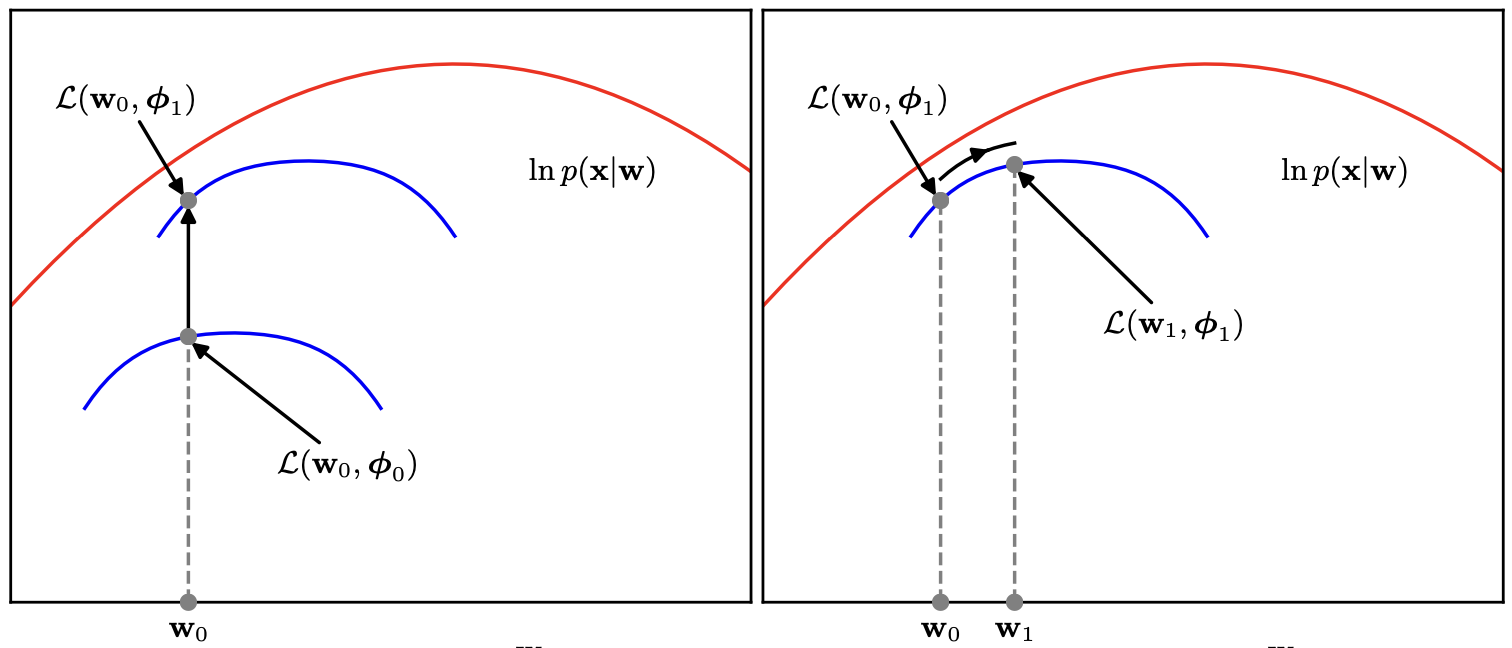
\includegraphics[width=\linewidth]{figs/em_bishop4}
	\end{figure}
		
	\myfootnote{Bishop\,C. Deep Learning: Foundations and Concepts, 2024}
\end{frame}
%=======
\begin{frame}{Variational EM-algorithm}
	\begin{block}{ELBO}
		\vspace{-0.5cm}
		\[
			\log p(\bx| \btheta) = \cL_{\bphi, \btheta}(\bx) + KL(q(\bz | \bx, \bphi) || p(\bz|\bx, \btheta)) \geq \cL_{\bphi, \btheta}(\bx).
		\]
		\[
		 	\cL_{q, \btheta}(\bx) = \mathbb{E}_{q} \log p(\bx | \bz, \btheta) - KL(q(\bz | \bx, \bphi) || p(\bz))
		\]
		\vspace{-0.5cm}
	\end{block}
	\begin{itemize}
		\item \textbf{E-step}
		\vspace{-0.3cm}
		\[
			\bphi_k = \bphi_{k-1} + \left.\eta \cdot \nabla_{\bphi} \cL_{\bphi, \btheta_{k-1}}(\bx)\right|_{\bphi=\bphi_{k-1}},
		\]
		\vspace{-0.3cm} \\
		where $\bphi$~-- parameters of the variational posterior distribution $q(\bz | \bx, \bphi)$.
		\item \textbf{M-step}
		\[
			\btheta_k = \btheta_{k-1} + \left.\eta \cdot \nabla_{\btheta} \cL_{\bphi_k, \btheta}(\bx)\right|_{\btheta=\btheta_{k-1}},
		\]
		where $\btheta$~-- parameters of the generative distribution $p(\bx | \bz, \btheta)$.
	\end{itemize}
	Now all that is left is to obtain \textbf{unbiased} Monte Carlo estimates of the gradients: $\nabla_{\bphi} \cL_{\bphi, \btheta}(\bx)$, $\nabla_{\btheta} \cL_{\bphi, \btheta}(\bx)$. 
\end{frame}
%=======
\subsection{ELBO gradients, reparametrization trick}
%=======
\begin{frame}{ELBO gradients, (M-step, $\nabla_{\btheta} \cL_{\bphi, \btheta}(\bx)$)}
	\vspace{-0.3cm}
	\[
	 	\cL_{q, \btheta}(\bx) = \mathbb{E}_{q} \log p(\bx | \bz, \btheta) - KL (q(\bz | \bx, \bphi) || p(\bz))
	\]
	\vspace{-0.5cm}
	\begin{block}{M-step: $\nabla_{\btheta} \cL_{\bphi, \btheta}(\bx)$}
		\vspace{-0.7cm}
		\begin{multline*}
			\nabla_{\btheta} \cL_{\bphi, \btheta}(\bx)
			= {\color{olive}\nabla_{\btheta}} \int q(\bz|\bx, \bphi) \log p(\bx|\bz, \btheta) d \bz =  \\
			= \int q(\bz|\bx, \bphi) {\color{olive}\nabla_{\btheta}} \log p(\bx|\bz, \btheta) d \bz \approx  \\
			\approx \nabla_{\btheta}\log p(\bx|\bz^*, \btheta), \quad \bz^* \sim q(\bz|\bx, \bphi).
		\end{multline*}
		\vspace{-0.9cm}
	\end{block}
	\begin{block}{Naive Monte-Carlo estimation}
		\vspace{-0.7cm}
		\[
			p(\bx | \btheta) = \int p(\bx | \bz, \btheta) p(\bz) d\bz \approx \frac{1}{K} \sum_{k=1}^{K} p(\bx | \bz_k, \btheta), \quad \bz_k \sim p(\bz).
		\]
		\vspace{-0.5cm} 
	\end{block}
	The variational posterior $q(\bz|\bx, \bphi)$ assigns typically more probability mass in a smaller region than the prior $p(\bz)$. 
	\myfootnotewithlink{https://jmtomczak.github.io/blog/4/4\_VAE.html}{image credit: https://jmtomczak.github.io/blog/4/4\_VAE.html}
\end{frame}
%=======
\begin{frame}{ELBO gradients, (E-step, $\nabla_{\bphi} \cL_{\bphi, \btheta}(\bx)$)}
	\begin{block}{E-step: $\nabla_{\bphi} \cL_{\bphi, \btheta}(\bx)$}
		Difference from M-step: density function $q(\bz| \bx, \bphi)$ depends on the parameters $\bphi$, it is impossible to use the Monte-Carlo estimation:
		\begin{align*}
			\nabla_{\bphi} \cL_{\bphi, \btheta}(\bx) &= {\color{olive}\nabla_{\bphi}} \int q(\bz | \bx, \bphi)\log p(\bx | \bz, \btheta) d \bz - \nabla_{\bphi} KL(q(\bz | \bx, \bphi) || p(\bz)) \\
			& {\color{violet}\neq} \int q(\bz | \bx, \bphi) {\color{olive}\nabla_{\bphi}} \log p(\bx | \bz, \btheta) d \bz - \nabla_{\bphi} KL(q(\bz | \bx, \bphi) || p(\bz))
		\end{align*}
	\end{block}
	\vspace{-0.5cm}
	\begin{block}{Reparametrization trick (LOTUS trick)} 
		Suppose that $\bz \sim q(\bz | \bx, \bphi)$ is a random variable that is induced by the random variable $\bepsilon \sim p(\bepsilon)$ using the deterministic transform $\bz = \bg_{\bphi}(\bx, \bepsilon)$. Then
		\[
			\bbE_{\bz \sim q(\bz | \bx, \bphi)} \bff(\bz) = \bbE_{\bepsilon \sim p(\bepsilon)} \bff(\bg_{\bphi}(\bx, \bepsilon))
		\]
		Note that LHS takes the expectation by the parametric distribution $q(\bz | \bx, \bphi)$ and the RHS uses non-parametric distribution $p(\bepsilon)$.
	\end{block}
\end{frame}
%=======
\begin{frame}{ELBO gradients, (E-step, $\nabla_{\bphi} \cL_{\bphi, \btheta}(\bx)$)}
	\begin{block}{Reparametrization trick (LOTUS trick)} 
		\vspace{-0.7cm}
		\begin{multline*}
			\nabla_{\bphi}\int q(\bz|\bx, \bphi) \bff(\bz) d\bz = {\color{olive}\nabla_{\bphi}} \int p(\bepsilon)  \bff(\bg_{\bphi}(\bx, \bepsilon)) d\bepsilon  \\ = \int p(\bepsilon) {\color{olive}\nabla_{\bphi}} \bff(\bg_{\bphi}(\bx, \bepsilon)) d\bepsilon \approx \nabla_{\bphi} \bff(\bg_{\bphi}(\bx, \bepsilon^*)),
		\end{multline*}
		\vspace{-0.5cm} \\
		where $\bepsilon^* \sim p(\bepsilon)$.

	\end{block}
	\begin{block}{Variational assumption} 
		\vspace{-0.3cm}
		\[
			p(\bepsilon) = \mathcal{N}(0, \bI); \quad \bz = \bg_{\bphi}(\bx, \bepsilon) = \bsigma_{\bphi}(\bx) \odot \bepsilon + \bmu_{\bphi}(\bx);
		\]
		\[
			q(\bz| \bx, \bphi) = \cN (\bmu_{\bphi}(\bx), \bsigma^2_{\bphi}(\bx)).
		\]
		Here $\bmu_{\bphi}(\cdot), \bsigma_{\bphi}(\cdot)$ are parameterized functions (outputs of neural network). \\
		We will say that $q(\bz| \bx, \bphi) = \text{NN}_e(\bx, \bphi)$ is the \textbf{encoder}.
	\end{block}
\end{frame}
%=======
\begin{frame}{ELBO gradient (E-step, $\nabla_{\bphi} \cL_{\bphi, \btheta}(\bx)$)}
	\vspace{-0.3cm}
	\[
		\nabla_{\bphi} \cL_{\bphi, \btheta}(\bx) = {\color{violet}\nabla_{\bphi} \int q(\bz | \bx, \bphi)\log p(\bx | \bz, \btheta) d \bz} - {\color{teal}\nabla_{\bphi} KL(q(\bz | \bx, \bphi) || p(\bz))}
	\]
	\vspace{-0.3cm}
	\begin{block}{Reconstruction term}
		\vspace{-0.7cm}
		\begin{multline*}
			 {\color{violet}\nabla_{\bphi} \int q(\bz | \bx, \bphi)\log p(\bx | \bz, \btheta) d \bz} = \int p(\bepsilon) \nabla_{\bphi} \log p(\bx | \bg_{\bphi}(\bx, \bepsilon), \btheta) d\bepsilon \approx \\
			 \approx \nabla_{\bphi} \log p\left(\bx | \bsigma_{\bphi}(\bx) \odot \bepsilon^* + \bmu_{\bphi}(\bx), \btheta\right), \quad \text{where } \bepsilon^* \sim \cN(0, \bI)
		\end{multline*}
		\vspace{-0.5cm} \\
		Let the generative distibution $p(\bx | \bz, \btheta)$ be the neural network. \\
		We will say that $p(\bx | \bz, \btheta) = \text{NN}_d(\bz, \btheta)$ is the \textbf{decoder}.
	\end{block}
	\begin{block}{KL term}
		$p(\bz)$ is the prior distribution on the latent variables $\bz$. Let assume $p(\bz) = \cN (0, \bI)$.
		\[
			{\color{teal}\nabla_{\bphi} KL(q(\bz | \bx, \bphi) || p(\bz))} = \nabla_{\bphi} KL\left( \cN (\bmu_{\bphi}(\bx), \bsigma^2_{\bphi}(\bx)) || \cN (0, \bI) \right)
		\]
		This expression has analytical formula.
	\end{block}
\end{frame}
%=======
\section{Variational autoencoder (VAE)}
%=======
\begin{frame}{Generative models zoo}
	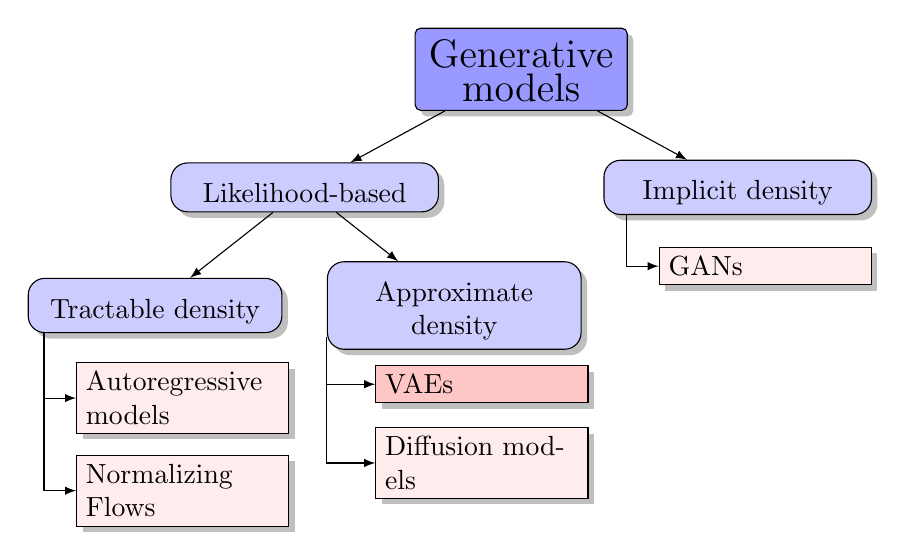
\begin{tikzpicture}[
		basic/.style  = {draw, text width=2cm, drop shadow, rectangle},
		root/.style   = {basic, rounded corners=2pt, thin, text height=1.1em, text width=7em, align=center, fill=blue!40},
		level 1/.style={sibling distance=55mm},
		level 2/.style = {basic, rounded corners=6pt, thin, align=center, fill=blue!20, text height=1.1em, text width=9em, sibling distance=38mm},
		level 3/.style = {basic, rounded corners=6pt, thin,align=center, fill=blue!20, text width=8.5em},
		level 4/.style = {basic, thin, align=left, fill=pink!30, text width=7em},
		level 5/.style = {basic, thin, align=left, fill=pink!90, text width=7em},
		edge from parent/.style={->,draw},
		>=latex]
		
		% root of the the initial tree, level 1
		\node[root] {\Large Generative models}
		% The first level, as children of the initial tree
		child {node[level 2] (c1) {Likelihood-based}
			child {node[level 3] (c11) {Tractable density}}
			child {node[level 3] (c12) {Approximate density}}
		}
		child {node[level 2] (c2) {Implicit density}};
		
		% The second level, relatively positioned nodes
		\begin{scope}[every node/.style={level 5}]
			\node [below of = c12, xshift=10pt] (c121) {VAEs};
		\end{scope}
		
		% The second level, relatively positioned nodes
		\begin{scope}[every node/.style={level 4}]
			\node [below of = c11, yshift=-5pt, xshift=10pt] (c111) {Autoregressive models};
			\node [below of = c111, yshift=-5pt] (c112) {Normalizing Flows};
			
			\node [below of = c121] (c122) {Diffusion models};
			\node [below of = c2, xshift=10pt] (c21) {GANs};
			
		\end{scope}
		
		
		% lines from each level 1 node to every one of its "children"
		\foreach \value in {1,2}
		\draw[->] (c11.194) |- (c11\value.west);
		
		\foreach \value in {1,2}
		\draw[->] (c12.194) |- (c12\value.west);
		
		\draw[->] (c2.194) |- (c21.west);
		
	\end{tikzpicture}
\end{frame}
%=======
\begin{frame}{Variational autoencoder (VAE)}
	\begin{block}{Training (EM-algorithm)}
		\begin{itemize}
			\item pick random sample $\bx_i, i \sim \text{Uniform}\{1, n\}$ (or batch).
			\item compute the objective (using reparametrization trick):
			\vspace{-0.3cm}
			\[
				\bepsilon^* \sim p(\bepsilon); \quad \bz^* = \bg_{\bphi}(\bx, \bepsilon^*);
			\]
			\[
				\cL_{\bphi, \btheta}(\bx) \approx  \log p(\bx | \bz^*, \btheta) - KL(q(\bz^* | \bx, \bphi) || p(\bz^*)).
			\]
			\item make gradient step using stochastic gradients w.r.t. $\bphi$ and $\btheta$ via autograd
		\end{itemize}
	\end{block}
	\begin{block}{Inference}
		\begin{itemize}
			\item sample $\bz^*$ from the prior distribution $p(\bz)$ ($\cN(0, \bI)$);
			\item sample from the decoder $p(\bx | \bz^*, \btheta)$.
		\end{itemize}
	\end{block}
	\textbf{Note:} you do not need the encoder $q(\bz | \bx, \bphi)$ during the generation.
\end{frame}
%=======
\begin{frame}{Variational Autoencoder}
	\vspace{-0.3cm}
	\[
	 	\cL_{q, \btheta}(\bx) = \mathbb{E}_{q} \log p(\bx | \bz, \btheta) - KL (q(\bz | \bx, \bphi) || p(\bz))
	\]
	\vspace{-0.5cm}
	\begin{minipage}[t]{0.6\columnwidth}
		\begin{figure}[h]
			\centering
			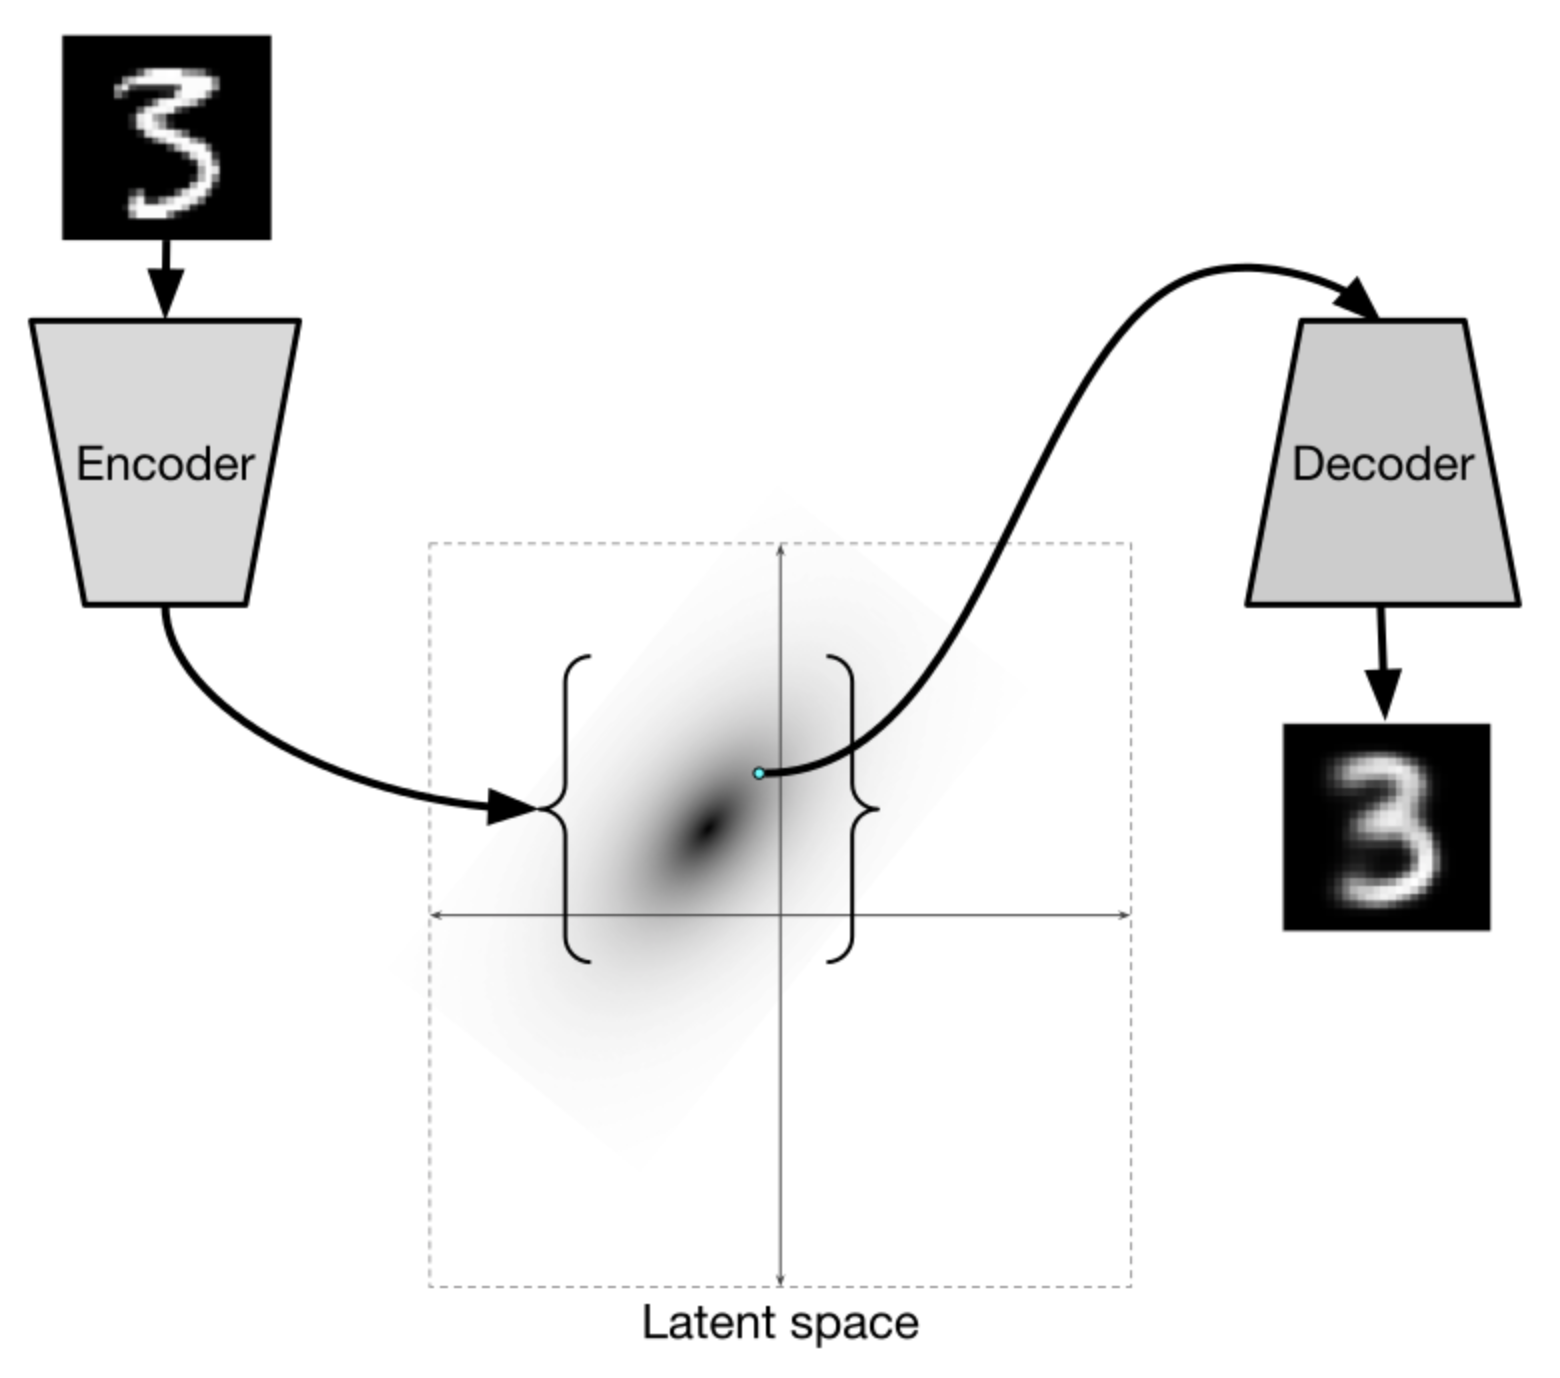
\includegraphics[width=\linewidth]{figs/VAE}
		\end{figure}
	\end{minipage}%
	\begin{minipage}[t]{0.4\columnwidth}
		\begin{figure}[h]
			\centering
			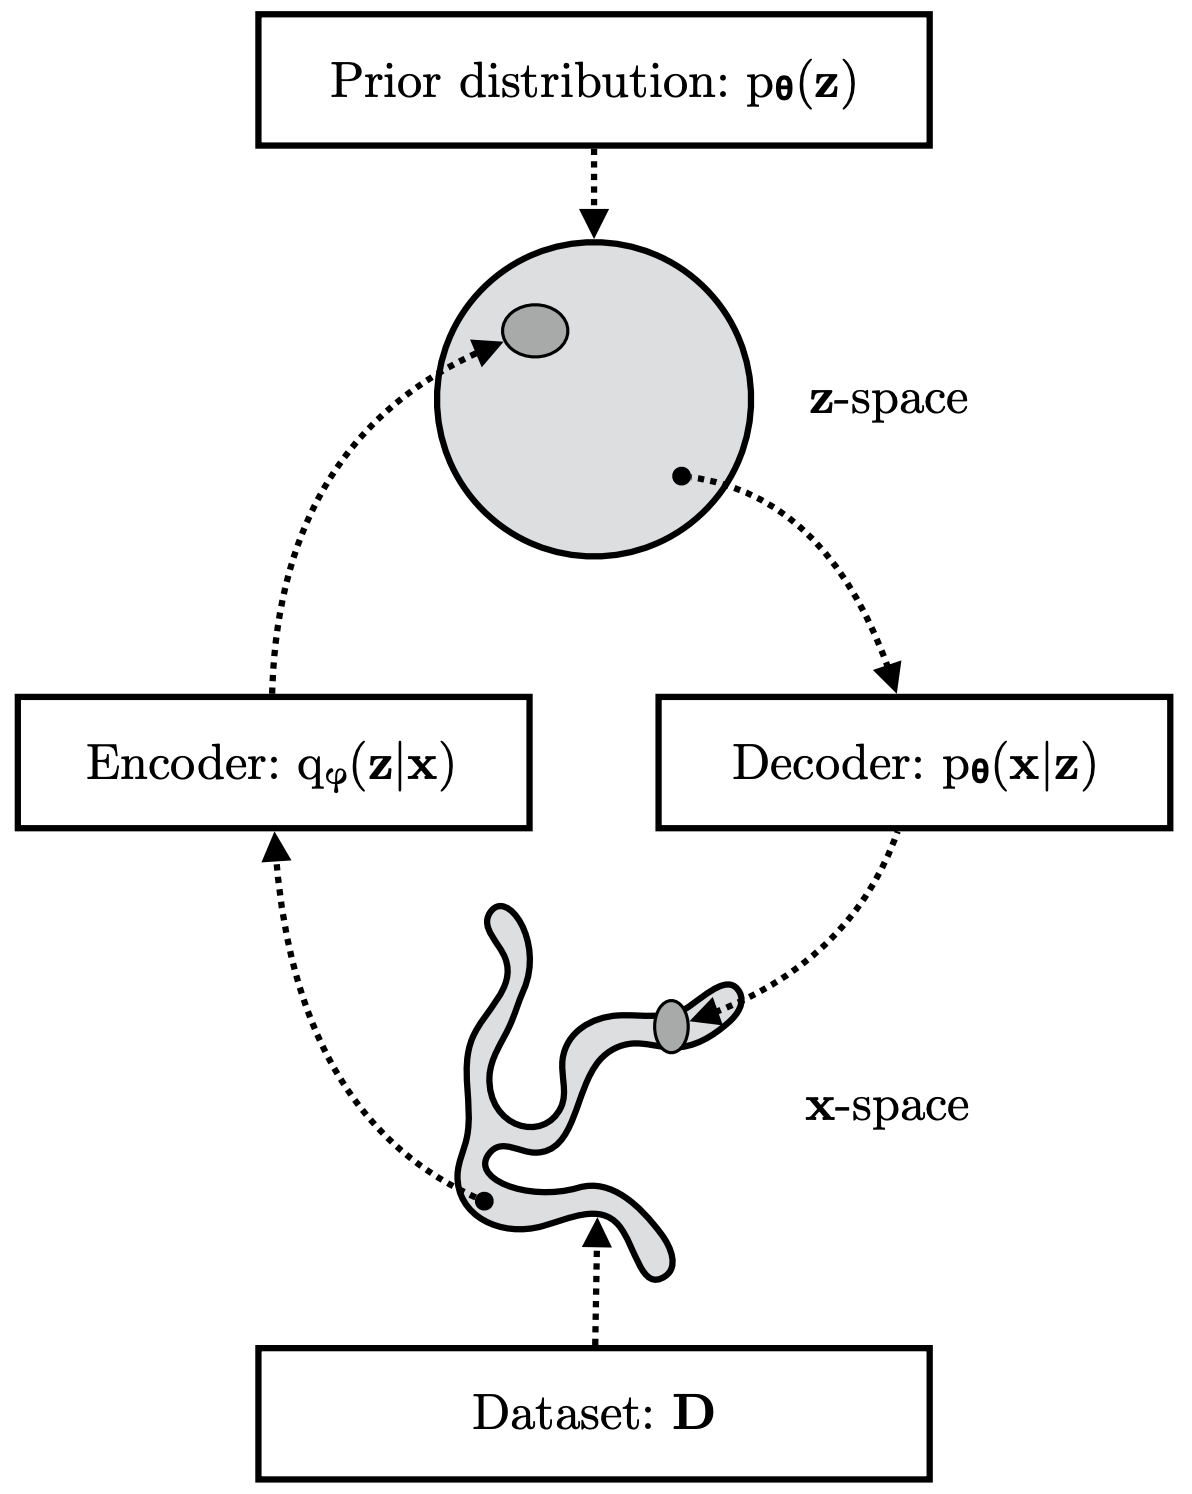
\includegraphics[width=\linewidth]{figs/vae_scheme}
		\end{figure}
	\end{minipage}
	\myfootnote{\href{http://ijdykeman.github.io/ml/2016/12/21/cvae.html}{image credit: http://ijdykeman.github.io/ml/2016/12/21/cvae.html} \\ \href{https://arxiv.org/abs/1906.02691}{Kingma D. P., Welling M. An introduction to variational autoencoders, 2019}}
\end{frame}
%=======
\begin{frame}{Variational autoencoder (VAE)}
	\begin{itemize}
		\item Encoder $q(\bz | \bx, \bphi) = \text{NN}_e(\bx, \bphi)$ outputs $\bmu_{\bphi}(\bx)$ and $\bsigma_{\bphi}(\bx)$.
		\item Decoder $p(\bx | \bz, \btheta) = \text{NN}_d(\bz, \btheta)$ outputs parameters of the sample distribution.
	\end{itemize}
	\begin{figure}[h]
		\centering
		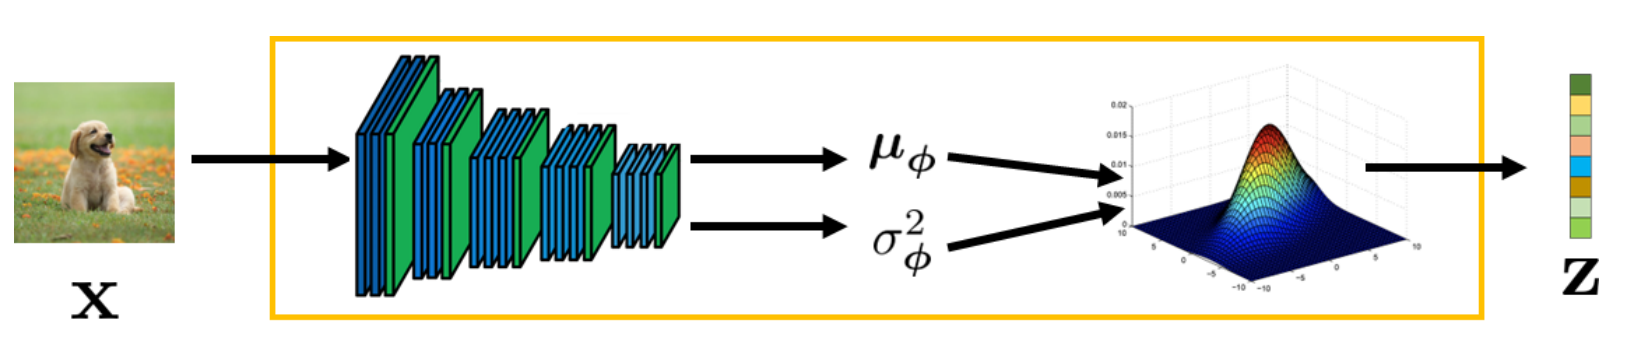
\includegraphics[width=0.7\linewidth]{figs/vae-encoder}
	\end{figure}
	\begin{figure}[h]
		\centering
		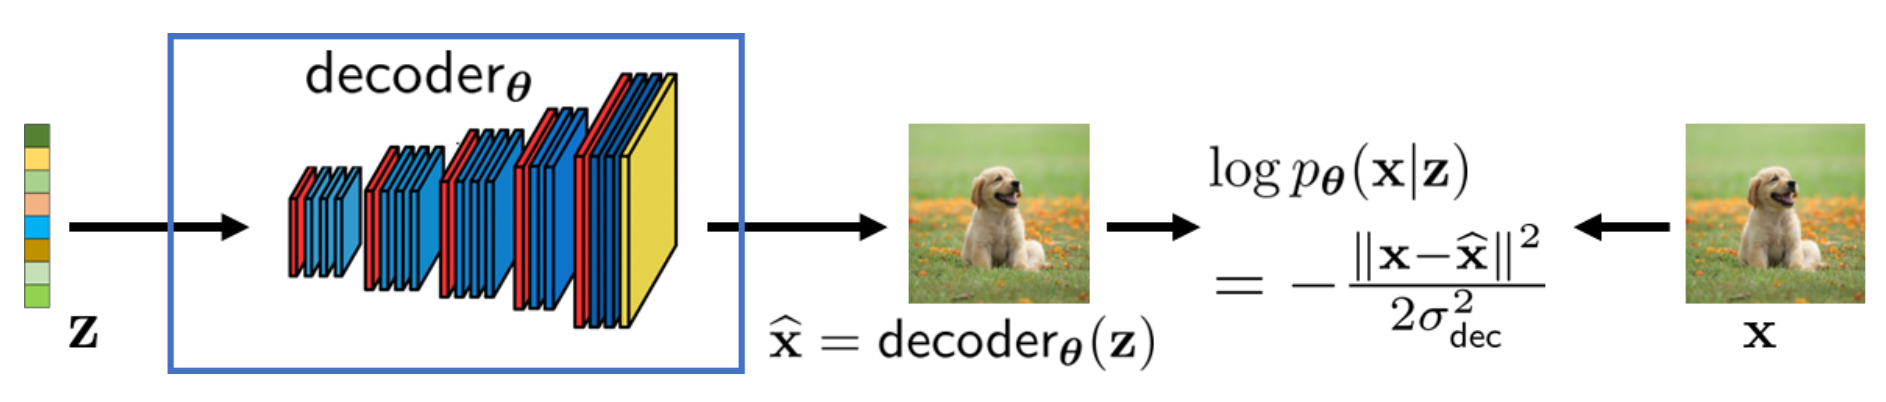
\includegraphics[width=0.9\linewidth]{figs/vae-decoder}
	\end{figure}
	
	\myfootnotewithlink{https://arxiv.org/pdf/2403.18103}{Chan S. Tutorial on Diffusion Models for Imaging and Vision, 2024}
\end{frame}
%=======
\begin{frame}{VAE vs Normalizing flows}
	\begin{table}[]
		\begin{tabular}{l|c|c}
			& \textbf{VAE} & \textbf{NF} \\ \hline
			\textbf{Objective} & ELBO $\cL$ & Forward KL/MLE \\ \hline
			\textbf{Encoder} & \shortstack{stochastic \\ $\bz \sim q (\bz | \bx, \bphi)$} &  \shortstack{\\ deterministic \\ $\bz = \bff_{\btheta}(\bx)$ \\ $q(\bz | \bx, \btheta) = \delta(\bz - \bff_{\btheta}(\bx))$}  \\ \hline
			\textbf{Decoder} & \shortstack{stochastic \\ $\bx \sim p (\bx | \bz, \btheta)$} & \shortstack{\\ deterministic \\ $\bx = \bg_{\btheta}(\bz)$ \\ $ p(\bx | \bz, \btheta) = \delta(\bx - \bg_{\btheta}(\bz))$} \\ \hline
			\textbf{Parameters}  & $\bphi, \btheta$ & $\btheta \equiv \bphi$\\ 
		\end{tabular}
	\end{table}
	\begin{block}{Theorem}
		MLE for normalizing flow is equivalent to maximization of ELBO for VAE model with deterministic encoder and decoder:
		\vspace{-0.3cm}
		\[
			p(\bx | \bz, \btheta) = \delta (\bx - \bff^{-1}_{\btheta}(\bz)) = \delta (\bx - \bg_{\btheta}(\bz));
		\]
		\[
			q(\bz | \bx, \btheta) = \delta (\bz - \bff_{\btheta}(\bx)).
		\]
	\end{block}
	\myfootnotewithlink{https://arxiv.org/abs/2007.02731}{Nielsen D., et al. SurVAE Flows: Surjections to Bridge the Gap between VAEs and Flows, 2020}
\end{frame}
%=======
\section{Discrete VAE latent representations}
%=======
\begin{frame}{Discrete VAE latents}
	\begin{block}{Motivation}
		\begin{itemize}
			\item Previous VAE models had \textbf{continuous} latent variables $\bz$.
			\item \textbf{Discrete} representations $\bz$ are potentially a more natural fit for many of the modalities.
			\item Powerful autoregressive models (like PixelCNN) have been developed for modelling distributions over discrete variables.
			\item All cool transformer-like models work with discrete tokens.
		\end{itemize}
	\end{block}
	\begin{block}{ELBO}
		\vspace{-0.3cm}
		\[
			\cL_{\bphi, \btheta}(\bx)  = \mathbb{E}_{q(\bz | \bx, \bphi)} \log p(\bx | \bz , \btheta) - KL(q(\bz| \bx, \bphi) || p(\bz)) \rightarrow \max_{\bphi, \btheta}.
		\]
		\vspace{-0.5cm}
	\end{block}
	\begin{itemize}
		\item Reparametrization trick to get unbiased gradients.
		\item Normal assumptions for $q(\bz | \bx, \bphi)$ and $p(\bz)$ to compute KL analytically.
	\end{itemize}
\end{frame}
%=======
\begin{frame}{Discrete VAE latents}
	\begin{block}{Assumptions}
		\begin{itemize}
			\item Let $c \sim \text{Categorical}(\bpi)$, where 
			\vspace{-0.6cm}
			\[
			\bpi = (\pi_1, \dots, \pi_K), \quad \pi_k = P(c = k), \quad \sum_{k=1}^K \pi_k = 1.
			\]
			\vspace{-0.6cm}
			\item Let VAE model has discrete latent representation $c$ with prior $p(c) = \text{Uniform}\{1, \dots, K\}$.
		\end{itemize}
	\end{block}
	\begin{block}{ELBO}
		\vspace{-0.5cm}
		\[
			\cL_{\bphi, \btheta}(\bx)  = \mathbb{E}_{q(c | \bx, \bphi)} \log p(\bx | c, \btheta) - {\color{olive} KL(q(c| \bx, \bphi) || p(c))} \rightarrow \max_{\bphi, \btheta}.
		\]
	\end{block}
	\vspace{-1.0cm}
	{\small
	\begin{multline*}
		{\color{olive} KL(q(c| \bx, \bphi) || p(c))} = \sum_{k=1}^K q(k | \bx, \bphi) \log \frac{q(k | \bx, \bphi)}{p(k)} = 
		\\ = \color{violet}{\sum_{k=1}^K q(k | \bx, \bphi) \log q(k | \bx, \bphi)}  \color{teal}{- \sum_{k=1}^K q(k | \bx, \bphi) \log p(k)}  = \\ = \color{violet}{- H(q(c | \bx, \bphi))} + \color{teal}{\log K}. 
	\end{multline*}
	}
\end{frame}
%=======
\begin{frame}{Discrete VAE latents}
	\vspace{-0.3cm}
	\[
		\cL_{\bphi, \btheta}(\bx)  = \mathbb{E}_{q(c | \bx, \bphi)} \log p(\bx | c, \btheta) + H(q(c | \bx, \bphi)) - \log K \rightarrow \max_{\bphi, \btheta}.
	\]
	\vspace{-0.3cm}
	\begin{itemize}
		\item Our encoder should output discrete distribution $q(c | \bx, \bphi)$.
		\item We need the analogue of the reparametrization trick for the discrete distribution $q(c | \bx, \bphi)$.
		\item Our decoder $p(\bx | c, \btheta)$ should input discrete random variable $c$.
	\end{itemize}
	\begin{figure}[h]
		\centering
		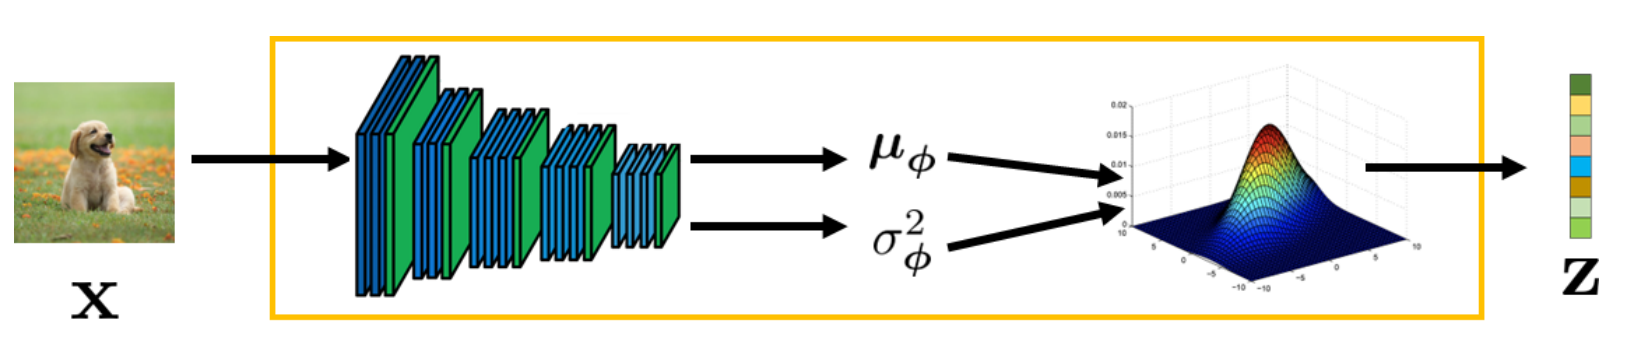
\includegraphics[width=0.7\linewidth]{figs/vae-encoder}
	\end{figure}
	\begin{figure}[h]
		\centering
		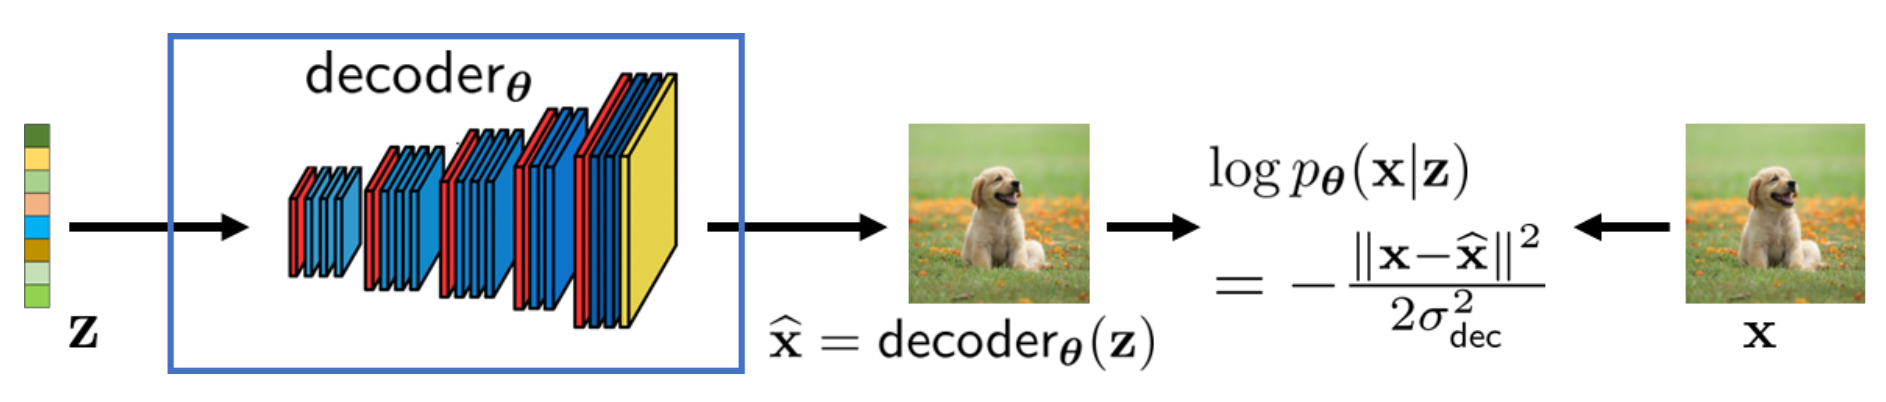
\includegraphics[width=0.9\linewidth]{figs/vae-decoder}
	\end{figure}
	\myfootnotewithlink{https://arxiv.org/pdf/2403.18103}{Chan S. Tutorial on Diffusion Models for Imaging and Vision, 2024}
\end{frame}
%=======
\begin{frame}{Summary}
	\begin{itemize}
		\item Amortized variational inference allows to efficiently compute the stochastic gradients for ELBO using Monte-Carlo estimation.
		\vfill
		\item The reparametrization trick gets unbiased gradients w.r.t. the variational posterior distribution $q(\bz | \bx, \bphi)$.
		\vfill
		\item The VAE model is an LVM with two neural network: stochastic encoder $q(\bz | \bx, \bphi)$ and stochastic decoder $p(\bx | \bz, \btheta)$.
		\vfill
		\item NF models could be treated as VAE model with deterministic encoder and decoder.
		\vfill
		\item Discrete VAE representations is a natural form of latent variables.
	\end{itemize}
\end{frame}
%=======
\end{document} 